% ==========================================================================================
% ==========================================================================================
% ==========================================================================================

\documentclass[10pt]{beamer}
    % ==========================================================================================
% ==========================================================================================
% ==========================================================================================

% Basic Setup

		\mode<presentation>
				{
					  \usetheme{Madrid}    % Hanover  
					  \usecolortheme{dolphin} % rose
					  \usefonttheme{serif}   % structurebold
					  \setbeamertemplate{navigation symbols}{} 
					  \setbeamertemplate{footline}{}   
					  \setbeamertemplate{frametitle}{\centering\normalsize\bfseries\slshape\insertframetitle\par\vskip-7pt\hrulefill} 
                                          \setbeamercolor{alerted text}{fg=blue}
				} 
               % \addtobeamertemplate{footline}{\vskip-1cm\hskip17pt\insertframenumber\,/\,\inserttotalframenumber\kern1em\vskip2pt}
                
% ==========================================================================================
% ==========================================================================================
% ==========================================================================================

% Packages
             %sansmathfonts

        \usepackage[T1]{fontenc}
		\usepackage{microtype,verbatim,parskip,graphicx,siunitx,nicefrac,booktabs,textpos,mathrsfs} %,rotating,textcomp 
		\usepackage[version=4]{mhchem}
		\usepackage{chemfig}\setchemfig{atom sep=2.5em}

		% Note: sansmathfonts redefines ALL math (including Greek) as sans-serif.
		%       we want this for Greek letters that look nice when mixed with a sans-serif font like helvet.
		%       however, this also forces Arabic numerals into cmu-serif for math mode, which looks bad next to helvet text.
		%       so below, we activate helvet as our main font, then add helvet serif math too.
		%       for some reason, this does not affect the Greek, which is why we need sansmathfonts beforehand.   

		%\usepackage{helvet}
		%\usepackage[helvet]{sfmath}

% ==========================================================================================
% ==========================================================================================
% ==========================================================================================

% Definitions

	    \def\deg{$^{\circ}$}
	    \def\tild{$\sim$}
	    \def\dg{$\Delta G$}
	    \def\electron{e$^-$}
	    \def\Ecell{$\mathscr{E}_{\textnormal{cell}}$}
	    \def\Enotcell{$\mathscr{E}^{\circ}_{\textnormal{cell}}$}
	    \def\Enot{$\mathscr{E}^{\circ}$}
	    \def\not{^\circ}
	    \def\Ka{$K_{\textnormal{a}}$}
	    \def\Ksp{$K_{\textnormal{sp}}$}
	    \def\Keq{$K_{\textnormal{eq}}$}
	    \def\pKa{p$K_{\textnormal{a}}$}
	    \def\dipole{+\hspace*{-3mm}$\longrightarrow$}
	    \def\cmi{cm$^{-1}$}
	    \def\cd{$\cdot$}
	    \def\dd{\end{document}} % useful for debugging

% ==========================================================================================
% ==========================================================================================
% ==========================================================================================

% Commands 

		\newcommand*\unit[1]{\textnormal{ #1}}
		% provides \obox{0}{0}{1cm}{1cm}   where: x y wd ht
		\newcommand\obox[4]{\pgfsetfillopacity{0.5}\begin{textblock}{}(#1,#2)\setlength\textwidth{#3}
		\begin{beamercolorbox}{block body}\vspace*{#4}\end{beamercolorbox}\end{textblock}\pgfsetfillopacity{1}}

		% provides \tbox{0}{0}{text} where: x y text
		\newcommand\tbox[3]{\begin{textblock}{8}(#1,#2)#3\end{textblock}}

% ==========================================================================================
% ==========================================================================================
% ==========================================================================================






















% ==========================================================================================
% ==========================================================================================
% ==========================================================================================

\def\mylabel{Chapter}
\def\mydeckno{17}

% ==========================================================================================
% ==========================================================================================
% ==========================================================================================

\title{FEP/GBSA\\and the\\Approximated Generalized\\Born Potential}
\author{John Terhorst}
\institute{Department of Chemistry\\Yale University}
\date{\scriptsize Monday, September 26, 2011}

% ==========================================================================================
% ==========================================================================================
% ==========================================================================================

\begin{document}

% ==========================================================================================
% ==========================================================================================
% ==========================================================================================

\begin{frame}

    \vspace*{-1cm}\titlepage
    \vspace*{-1cm}{\centering \includegraphics[scale=0.15]{figures/pdf/yalelogo.pdf}\\}

\end{frame}

% ==========================================================================================
% ==========================================================================================
% ==========================================================================================

\section{Overview}

% ==========================================================================================
% ==========================================================================================
% ==========================================================================================

\begin{frame}{Overview}

\begin{itemize}
    \item Background
    \begin{itemize}
    \item Explicit versus implicit water models.
    \item The generalized Born/ surface area (GB/SA) solvation model. 
    \item GB/SA in protein simulations.
    \end{itemize}
    \item Implementing free-energy perturbation (FEP) with GB/SA
    \begin{itemize}
    \item Challenges with FEP/GBSA.
    \item Energy trajectories and free energies of hydration.
    \end{itemize}
    \item Making in better
    \begin{itemize}
    \item The approximated generalized Born potential. 
    \item Statistical significance of the approximation.
    \item Chlorine scan.
    \end{itemize}
\end{itemize}

\end{frame}

% ==========================================================================================
% ==========================================================================================
% ==========================================================================================

\section{Background}

% ==========================================================================================
% ==========================================================================================
% ==========================================================================================

\subsection{Solvent models}

% ==========================================================================================
% ==========================================================================================
% ==========================================================================================

\begin{frame}[t]{Explicit solvent models}

\begin{itemize}
    \item The classical approach to modeling solvents.
    \begin{itemize}
    \item Explicit treatment of all atoms.
    \item Each atom is defined with its own coordinates, van der Waals radius, partial charge, and polarizability (if applicable).
    \item All interactions between all atoms within their solvation shells or within a pre-defined cutoff are considered.
    \end{itemize}
    \item Rely on molecular mechanics, rather than quantum mechanics.
    \begin{itemize}
    \item Parameters are usually based on quantum mechanical calculations.
    \end{itemize}
    \begin{center}
    \includegraphics[scale=0.2]{figures/waters.png}
    \end{center}
    \item A change in the liquid structure as a result of a perturbation to the system necessitates that all interactions be relaxed, or equilibrated, to once again achieve the system's low-energy state.
\end{itemize}
\end{frame}

% ==========================================================================================
% ==========================================================================================
% ==========================================================================================

\begin{frame}[t]{Implicit solvent models}

\begin{itemize}
    \item Designed to curtail some problems of the explicit approach to representing solvent, by abstracting solvent molecules into a dielectric continuum with the average properties of the liquid.
	\begin{center}
	\includegraphics[scale=0.2]{figures/implicit.png}
	\end{center}
	\item The average influence of the solvent is determined by direct estimation of the free energy of solvation.
	\item Solvent is always equilibrated, by definition.
	\begin{itemize}
    \item No sampling of solvent is required.
    \item Avoids errors arising from incomplete sampling of solvent configurations.
    \end{itemize}
    \item Dedicated sampling of solutes.
    \item Simplification of system setup.
\end{itemize}
\end{frame}

% ==========================================================================================
% ==========================================================================================
% ==========================================================================================

\subsection{The GB/SA solvation model}

% ==========================================================================================
% ==========================================================================================
% ==========================================================================================

\begin{frame}[t]{The GB/SA solvation model}

\begin{itemize}
    \item Details: Still, W. C.; Tempczyk, A.; Hawley, R. C.; Hendrickson, T. (1990)\footnote{\textit{J.\ Am.\ Chem.\ Soc.} \textbf{1990}, \textit{112}, 6127.}
\end{itemize}
%
\begin{equation*}
G_\textnormal{sol} = G_\textnormal{cav} + G_\textnormal{vdW} + G_\textnormal{pol}  
\end{equation*}

\begin{equation*}
G_\textnormal{cav} + G_\textnormal{vdW} = G_\textnormal{np} = \sum_i\sigma_i SA_i
\end{equation*}

\begin{equation*}
G_\textnormal{pol} = -166.0\left(1-\frac{1}{\varepsilon}\right)\frac{q^2}{\alpha}
\end{equation*}

\begin{equation*}
G_\textnormal{pol} = -166.0\left(1-\frac{1}{\varepsilon}\right)\sum_i\sum_j\frac{q_iq_j}{r^2_{ij}+\alpha^2_{ij}\exp(-r^2_{ij}/2\alpha^2_{ij})^{1/2}}
\end{equation*}

\begin{center}
\includegraphics[scale=0.179]{figures/pdf/bornradius.pdf}
\end{center}
\end{frame}

% ==========================================================================================
% ==========================================================================================
% ==========================================================================================

\begin{frame}[t]{The GB/SA solvation model}

\begin{itemize}
    \item Details: Qiu, D.; Shenkin, P. S.; Hollinger, F. P.; Still, W. C. (1997)\footnote{\textit{J.\ Phys.\ Chem.\ A} \textbf{1997}, \textit{101}, 3005.}
\end{itemize}

\vspace*{5mm}
\begin{equation*}
G^\prime_{\textnormal{pol},i} = \frac{-166.0}{R_{\textnormal{vdW},i}+\phi+P_1} + \sum^{1,2}\frac{P_2V_j}{r^4_{ij}} + \sum^{1,3}\frac{P_3V_j}{r^4_{ij}} + \sum^{1,\ge 4}\frac{P_4V_jCCF}{r^4_{ij}}
\end{equation*}

\vspace*{5mm}
\begin{center}
\includegraphics[scale=0.22]{figures/pdf/gpoli.pdf}
\end{center}
\end{frame}

% ==========================================================================================
% ==========================================================================================
% ==========================================================================================

\subsection{Repercussions in Monte Carlo simulations}

% ==========================================================================================
% ==========================================================================================
% ==========================================================================================

\begin{frame}[t]{Repercussions in Monte Carlo simulations}

\begin{center}
\includegraphics[scale=0.3]{figures/moves.png}
\end{center}

\vspace*{5mm}
\begin{itemize}
    \item The generalized Born energy is not pairwise decomposable:
    \begin{itemize}
    \item The Born radius of any given atom depends on the volume and position of every other atom in the system.
    \item All atom-pair energies are affected by every move in a Monte Carlo simulation, due to changes in Born radii of the pair's constituent atoms.
    \end{itemize}
    \item Therefore, all atom-pair energies must be calculated after every move in a Monte Carlo simulation.
\end{itemize}

\end{frame}

% ==========================================================================================
% ==========================================================================================
% ==========================================================================================

\begin{frame}[t]{GB/SA in simulations of proteins}

There is great appeal in employing implicit solvents in simulations of large
GB/SA solvation in protein simulations biomolecular systems, and many have done so in:

\begin{itemize}
    \item RNA hairpin unfolding\footnote{\textit{J.\ Mol.\ Biol.} \textbf{2002}, \textit{317}, 493.} (MD)
    \item Nucleic acid conformational dynamics\footnote{\textit{Biophys.\ J.} \textbf{2003}, \textit{85}, 790.} (MD)
    \item Determination of free-energy surfaces in peptides\footnote{\textit{Proteins} \textbf{2004}, \textit{56}, 310} (MD)
    \item Potential application of Monte Carlo sampling algorithms:
    \begin{itemize}
    \item Flexible docking\footnote{\textit{J.\ Comput.\ Chem.} \textbf{2004}, \textit{24}, 1637.}
    \item Concerted rotation with angles\footnote{\textit{J.\ Chem.\ Phys.} \textbf{2003}, \textit{118}, 4261.}
    \end{itemize}
\end{itemize}

Few have exploited GB/SA in rigorous Monte Carlo free-energy calculations
of binding affinities. Why not?

%\begin{center}
%\includegraphics[scale=0.3]{figures/frozen.png}
%\end{center}       

\end{frame}

% ==========================================================================================
% ==========================================================================================
% ==========================================================================================

\subsection{MC/FEP}

% ==========================================================================================
% ==========================================================================================
% ==========================================================================================

\begin{frame}[t]{Monte Carlo free-energy perturbation}

From perturbation theory, FEP is the methodology of choice for computation of relative free energies of binding for different ligands to a protein. Zwanzig\footnote{\textit{J.\ Chem.\ Phys.} \textbf{1954}, \textit{22}, 1420--1426} in 1954:

\begin{equation*}
\Delta G(A \rightarrow B) = G_\textnormal{B} - G_\textnormal{A} = -k_\textnormal{B}T\ln\left\langle\exp\left(-\frac{E_\textnormal{B}-E_\textnormal{A}}{k_\textnormal{B}T}\right)\right\rangle_{\textnormal{A}}
\end{equation*}

\begin{center}
\includegraphics[scale=0.7]{figures/cycle.pdf}
\end{center}

Perturbations are split into small increments.

3 energy calculations are performed for each accepted move...

\end{frame}


% ==========================================================================================
% ==========================================================================================
% ==========================================================================================

\section{Implementation}

\subsection{Technical challenges}

% ==========================================================================================
% ==========================================================================================
% ==========================================================================================

\begin{frame}{Technical challenges}

Our GB/SA implementation uses united-atom (UA) charges on saturated alkyl groups, but perturbations often require
UA charges $\longrightarrow$ AA charges or AA charges $\longrightarrow$ UA charges.

\bigskip
\begin{center}
\includegraphics[scale=0.8]{figures/ua-aa.pdf}
\end{center}
\begin{itemize}
\bigskip

\item Dummy atoms (SASA and Coulombic)
\item 1,2 and 1,3 terms are ignored for hydrogens on saturated carbons
\item Adjustment of volume due to atomic overlap can be problematic
\item Non-bonded terms are ignored for all hydrogens
\item Corrections to the initially assigned charges are made for N---O compounds

\end{itemize}

\end{frame}

% ==========================================================================================
% ==========================================================================================
% ==========================================================================================

\subsection{Test Cases}

% ==========================================================================================
% ==========================================================================================
% ==========================================================================================

\begin{frame}{Test cases: typical perturbation}

\begin{center}
\includegraphics[scale=0.22]{figures/typical.png}
\end{center}

\end{frame}

% ==========================================================================================
% ==========================================================================================
% ==========================================================================================

\section{Sample Data}

\subsection{Energy Components}

% ==========================================================================================
% ==========================================================================================
% ==========================================================================================

\begin{frame}{Energy components: chlorobenzene to benzene}

    \begin{columns}

        \begin{column}{0.65\textwidth}

\begin{center}
\hspace*{1cm}\includegraphics[scale=0.7]{figures/clhrxn.pdf}\\
\scalebox{.5}{\input{figures/clh-en/clh-en}}\hspace*{-1cm}\scalebox{.5}{\input{figures/clh-charge/clh-charge}}\\
\scalebox{.5}{\input{figures/clh-vol/clh-vol}}\hspace*{-1cm}\scalebox{.5}{\input{figures/clh-pol/clh-pol}}
\end{center} 

        \end{column}
        
        \begin{column}{0.3\textwidth}  
        
The challenge: large volume change; significant overlap; reversal of charge distribution.

\bigskip

The results: smooth perturbation of charge and volume; volume of C increases due to loss of overlap from Cl/H; charge reversal yields correct charges on benzene.


        \end{column}

    \end{columns}

\end{frame}

% ==========================================================================================
% ==========================================================================================
% ==========================================================================================

\begin{frame}{Energy components: cyanobenzene to fluorozene}

    \begin{columns}

        \begin{column}{0.65\textwidth}

\begin{center}
\hspace*{1cm}\includegraphics[scale=0.7]{figures/cnfrxn.pdf}\\
\scalebox{.5}{\input{figures/cnf-en/cnf-en}}\hspace*{-1cm}\scalebox{.5}{\input{figures/cnf-charge/cnf-charge}}\\
\scalebox{.5}{\input{figures/cnf-vol/cnf-vol}}\hspace*{-1cm}\scalebox{.5}{\input{figures/cnf-pol/cnf-pol}}
\end{center} 

        \end{column}
        
        \begin{column}{0.3\textwidth}  
        
The challenge: one dummy atom; significant overlap; reversal of charge distribution.

\bigskip

The results: smooth perturbation of charge; volume of C decreases due to emergence of F; dummy charge scales to zero, volume to zero by $\lambda = 0.6$ due to overlap.


        \end{column}

    \end{columns}

\end{frame}

% ==========================================================================================
% ==========================================================================================
% ==========================================================================================

\begin{frame}{Energy components: acetophenone to benzamide}

    \begin{columns}

        \begin{column}{0.65\textwidth}

\begin{center}
\hspace*{1cm}\includegraphics[scale=0.7]{figures/comenh2rxn.pdf}\\
\scalebox{.5}{\input{figures/comenh2-en/comenh2-en}}\hspace*{-1cm}\scalebox{.5}{\input{figures/comenh2-charge/comenh2-charge}}\\
\scalebox{.5}{\input{figures/comenh2-vol/comenh2-vol}}\hspace*{-1cm}\scalebox{.5}{\input{figures/comenh2-pol/comenh2-pol}}
\end{center} 

        \end{column}
        
        \begin{column}{0.3\textwidth}  
        
The challenge: three perturbations, one dummy atom; dispersion of charge; UA/AA conversion; slight geometry change.
\bigskip

The results: smooth dispersion of charge; dummy volume scales to zero by $\lambda = 0.5$ due to overlap, electrostatic contribution constant at zero.

        \end{column}

    \end{columns}

\end{frame}

% ==========================================================================================
% ==========================================================================================
% ==========================================================================================

\begin{frame}[t]{Free energies of solvation: TIP4P and GB/SA}

\begin{center}
\scalebox{.7}{\input{figures/corrall/corrall}}
\end{center}

GB/SA trajectories behaved more like gas-phase trajectories than TIP4P trajectories; GB/SA and gas-phase trajectories typically followed a more predictable path, whereas TIP4P trajectories often fluctuated, owing to variations in water molecule configurations.

\end{frame}

% ==========================================================================================
% ==========================================================================================
% ==========================================================================================

\section{Approximated Generalized Born Potential}

% ==========================================================================================
% ==========================================================================================
% ==========================================================================================

\begin{frame}{Approximated Generalized Born Potential}

How can we overcome the limitations of a standard GB/SA implementation in MC simulations?

\bigskip
\begin{center}
\includegraphics[scale=0.375]{figures/parts.png}
\end{center}

\end{frame}

% ==========================================================================================
% ==========================================================================================
% ==========================================================================================

\begin{frame}{Approximated Generalized Born Potential}

How can we overcome the limitations of a standard GB/SA implementation in MC simulations?

\begin{itemize}
    \item Assumption: the impact of a moving atom on the Born radius of a distant atom is small. 
    \item Don’t recalculate atom-pair energy after a move if:
\end{itemize}

\begin{enumerate}
    \item neither atom moved; and
    \item the Born radius of neither atom changed by more than a pre-specified amount (threshold) since the last accepted move.
\end{enumerate}

\begin{itemize}
    \item A large number of atom-pair energy calculations would be skipped 
    \item Should have a minimal effect on the resulting ensemble of energies.
\end{itemize} 
\end{frame}

% ==========================================================================================
% ==========================================================================================
% ==========================================================================================

\begin{center}
\includegraphics[angle=270,scale=0.33]{figures/pdf/flow1.pdf}
\end{center}

% ==========================================================================================
% ==========================================================================================
% ==========================================================================================

\subsection{Threshold}

% ==========================================================================================
% ==========================================================================================
% ==========================================================================================

\begin{frame}[t]{The impact of the threshold}

\begin{center}
\scalebox{.8}{\input{figures/nskip/nskip}}
\end{center}

\begin{itemize}
    \item Response curve is system specific but trivially generated.
    \item By $\tau = 0.005$ \AA, most pairs (95\%+) were being skipped.
\end{itemize}

\end{frame}

% ==========================================================================================
% ==========================================================================================
% ==========================================================================================

\subsection{Improved efficiency}

% ==========================================================================================
% ==========================================================================================
% ==========================================================================================

\begin{frame}[t]{Improved efficiency}

\begin{center}
\scalebox{.8}{% GNUPLOT: LaTeX picture with Postscript
\begingroup
  \makeatletter
  \providecommand\color[2][]{%
    \GenericError{(gnuplot) \space\space\space\@spaces}{%
      Package color not loaded in conjunction with
      terminal option `colourtext'%
    }{See the gnuplot documentation for explanation.%
    }{Either use 'blacktext' in gnuplot or load the package
      color.sty in LaTeX.}%
    \renewcommand\color[2][]{}%
  }%
  \providecommand\includegraphics[2][]{%
    \GenericError{(gnuplot) \space\space\space\@spaces}{%
      Package graphicx or graphics not loaded%
    }{See the gnuplot documentation for explanation.%
    }{The gnuplot epslatex terminal needs graphicx.sty or graphics.sty.}%
    \renewcommand\includegraphics[2][]{}%
  }%
  \providecommand\rotatebox[2]{#2}%
  \@ifundefined{ifGPcolor}{%
    \newif\ifGPcolor
    \GPcolortrue
  }{}%
  \@ifundefined{ifGPblacktext}{%
    \newif\ifGPblacktext
    \GPblacktextfalse
  }{}%
  % define a \g@addto@macro without @ in the name:
  \let\gplgaddtomacro\g@addto@macro
  % define empty templates for all commands taking text:
  \gdef\gplbacktext{}%
  \gdef\gplfronttext{}%
  \makeatother
  \ifGPblacktext
    % no textcolor at all
    \def\colorrgb#1{}%
    \def\colorgray#1{}%
  \else
    % gray or color?
    \ifGPcolor
      \def\colorrgb#1{\color[rgb]{#1}}%
      \def\colorgray#1{\color[gray]{#1}}%
      \expandafter\def\csname LTw\endcsname{\color{white}}%
      \expandafter\def\csname LTb\endcsname{\color{black}}%
      \expandafter\def\csname LTa\endcsname{\color{black}}%
      \expandafter\def\csname LT0\endcsname{\color[rgb]{1,0,0}}%
      \expandafter\def\csname LT1\endcsname{\color[rgb]{0,1,0}}%
      \expandafter\def\csname LT2\endcsname{\color[rgb]{0,0,1}}%
      \expandafter\def\csname LT3\endcsname{\color[rgb]{1,0,1}}%
      \expandafter\def\csname LT4\endcsname{\color[rgb]{0,1,1}}%
      \expandafter\def\csname LT5\endcsname{\color[rgb]{1,1,0}}%
      \expandafter\def\csname LT6\endcsname{\color[rgb]{0,0,0}}%
      \expandafter\def\csname LT7\endcsname{\color[rgb]{1,0.3,0}}%
      \expandafter\def\csname LT8\endcsname{\color[rgb]{0.5,0.5,0.5}}%
    \else
      % gray
      \def\colorrgb#1{\color{black}}%
      \def\colorgray#1{\color[gray]{#1}}%
      \expandafter\def\csname LTw\endcsname{\color{white}}%
      \expandafter\def\csname LTb\endcsname{\color{black}}%
      \expandafter\def\csname LTa\endcsname{\color{black}}%
      \expandafter\def\csname LT0\endcsname{\color{black}}%
      \expandafter\def\csname LT1\endcsname{\color{black}}%
      \expandafter\def\csname LT2\endcsname{\color{black}}%
      \expandafter\def\csname LT3\endcsname{\color{black}}%
      \expandafter\def\csname LT4\endcsname{\color{black}}%
      \expandafter\def\csname LT5\endcsname{\color{black}}%
      \expandafter\def\csname LT6\endcsname{\color{black}}%
      \expandafter\def\csname LT7\endcsname{\color{black}}%
      \expandafter\def\csname LT8\endcsname{\color{black}}%
    \fi
  \fi
  \setlength{\unitlength}{0.0500bp}%
  \begin{picture}(7200.00,5040.00)%
    \gplgaddtomacro\gplbacktext{%
      \csname LTb\endcsname%
      \put(946,880){\makebox(0,0)[r]{\strut{} 20}}%
      \csname LTb\endcsname%
      \put(946,1367){\makebox(0,0)[r]{\strut{} 30}}%
      \csname LTb\endcsname%
      \put(946,1854){\makebox(0,0)[r]{\strut{} 40}}%
      \csname LTb\endcsname%
      \put(946,2341){\makebox(0,0)[r]{\strut{} 50}}%
      \csname LTb\endcsname%
      \put(946,2828){\makebox(0,0)[r]{\strut{} 60}}%
      \csname LTb\endcsname%
      \put(946,3314){\makebox(0,0)[r]{\strut{} 70}}%
      \csname LTb\endcsname%
      \put(946,3801){\makebox(0,0)[r]{\strut{} 80}}%
      \csname LTb\endcsname%
      \put(946,4288){\makebox(0,0)[r]{\strut{} 90}}%
      \csname LTb\endcsname%
      \put(946,4775){\makebox(0,0)[r]{\strut{} 100}}%
      \csname LTb\endcsname%
      \put(1078,660){\makebox(0,0){\strut{} 0}}%
      \csname LTb\endcsname%
      \put(2509,660){\makebox(0,0){\strut{} 0.0001}}%
      \csname LTb\endcsname%
      \put(3941,660){\makebox(0,0){\strut{} 0.001}}%
      \csname LTb\endcsname%
      \put(5372,660){\makebox(0,0){\strut{} 0.01}}%
      \csname LTb\endcsname%
      \put(6803,660){\makebox(0,0){\strut{} 0.1}}%
      \put(250,2827){\rotatebox{-270}{\makebox(0,0){\strut{}Relative percent calculation time}}}%
      \put(3940,330){\makebox(0,0){\strut{}Threshold $\tau$ (\AA)}}%
    }%
    \gplgaddtomacro\gplfronttext{%
      \csname LTb\endcsname%
      \put(5816,4602){\makebox(0,0)[r]{\strut{}100 moves}}%
      \csname LTb\endcsname%
      \put(5816,4382){\makebox(0,0)[r]{\strut{}1000 moves}}%
      \csname LTb\endcsname%
      \put(5816,4162){\makebox(0,0)[r]{\strut{}2500 moves}}%
      \csname LTb\endcsname%
      \put(5816,3942){\makebox(0,0)[r]{\strut{}5000 moves}}%
    }%
    \gplbacktext
    \put(0,0){\includegraphics{figures/speedup/speedup}}%
    \gplfronttext
  \end{picture}%
\endgroup
}
\end{center}

\begin{itemize}
    \item Most speed-up is achieved between threshold values of 0.001 and 0.01 \AA
    \item Little additional benefit is afforded at larger values.
\end{itemize}
\end{frame}

% ==========================================================================================
% ==========================================================================================
% ==========================================================================================

\begin{frame}[t]{Improved efficiency}

\vspace*{-1cm}
\begin{center}
\hspace*{-.85cm}\scalebox{.5}{\input{figures/pies/pienot}\hspace*{-5.2cm}\input{figures/pies/piethr}\hspace*{-5.2cm}\input{figures/pies/pieabs}}\\
 No threshold \hspace*{1.1cm} With threshold \hspace*{1.7cm} Relative \\
{\small red = \texttt{CALCEGB}, green = \texttt{EXPJ}, cyan = \texttt{READ}, pink = time saved}
\end{center}

\begin{itemize}
    \item With $\tau = 0.1$ \AA
    \item Throughout the process of implementing the new code, we monitored performance statistics in order to gauge our progress and to identify bottlenecks in the code.  
    \item This also proved valuable in determining which coding methods were most efficient in cases where several possible coding methods were available. 
\end{itemize}

\end{frame}
% ==========================================================================================
% ==========================================================================================
% ==========================================================================================

\subsection{Accumulation of error}

% ==========================================================================================
% ==========================================================================================
% ==========================================================================================

\begin{frame}[t]{Drift: accumulation of error}

\begin{center}
\scalebox{.75}{% GNUPLOT: LaTeX picture with Postscript
\begingroup
  \makeatletter
  \providecommand\color[2][]{%
    \GenericError{(gnuplot) \space\space\space\@spaces}{%
      Package color not loaded in conjunction with
      terminal option `colourtext'%
    }{See the gnuplot documentation for explanation.%
    }{Either use 'blacktext' in gnuplot or load the package
      color.sty in LaTeX.}%
    \renewcommand\color[2][]{}%
  }%
  \providecommand\includegraphics[2][]{%
    \GenericError{(gnuplot) \space\space\space\@spaces}{%
      Package graphicx or graphics not loaded%
    }{See the gnuplot documentation for explanation.%
    }{The gnuplot epslatex terminal needs graphicx.sty or graphics.sty.}%
    \renewcommand\includegraphics[2][]{}%
  }%
  \providecommand\rotatebox[2]{#2}%
  \@ifundefined{ifGPcolor}{%
    \newif\ifGPcolor
    \GPcolortrue
  }{}%
  \@ifundefined{ifGPblacktext}{%
    \newif\ifGPblacktext
    \GPblacktextfalse
  }{}%
  % define a \g@addto@macro without @ in the name:
  \let\gplgaddtomacro\g@addto@macro
  % define empty templates for all commands taking text:
  \gdef\gplbacktext{}%
  \gdef\gplfronttext{}%
  \makeatother
  \ifGPblacktext
    % no textcolor at all
    \def\colorrgb#1{}%
    \def\colorgray#1{}%
  \else
    % gray or color?
    \ifGPcolor
      \def\colorrgb#1{\color[rgb]{#1}}%
      \def\colorgray#1{\color[gray]{#1}}%
      \expandafter\def\csname LTw\endcsname{\color{white}}%
      \expandafter\def\csname LTb\endcsname{\color{black}}%
      \expandafter\def\csname LTa\endcsname{\color{black}}%
      \expandafter\def\csname LT0\endcsname{\color[rgb]{1,0,0}}%
      \expandafter\def\csname LT1\endcsname{\color[rgb]{0,1,0}}%
      \expandafter\def\csname LT2\endcsname{\color[rgb]{0,0,1}}%
      \expandafter\def\csname LT3\endcsname{\color[rgb]{1,0,1}}%
      \expandafter\def\csname LT4\endcsname{\color[rgb]{0,1,1}}%
      \expandafter\def\csname LT5\endcsname{\color[rgb]{1,1,0}}%
      \expandafter\def\csname LT6\endcsname{\color[rgb]{0,0,0}}%
      \expandafter\def\csname LT7\endcsname{\color[rgb]{1,0.3,0}}%
      \expandafter\def\csname LT8\endcsname{\color[rgb]{0.5,0.5,0.5}}%
    \else
      % gray
      \def\colorrgb#1{\color{black}}%
      \def\colorgray#1{\color[gray]{#1}}%
      \expandafter\def\csname LTw\endcsname{\color{white}}%
      \expandafter\def\csname LTb\endcsname{\color{black}}%
      \expandafter\def\csname LTa\endcsname{\color{black}}%
      \expandafter\def\csname LT0\endcsname{\color{black}}%
      \expandafter\def\csname LT1\endcsname{\color{black}}%
      \expandafter\def\csname LT2\endcsname{\color{black}}%
      \expandafter\def\csname LT3\endcsname{\color{black}}%
      \expandafter\def\csname LT4\endcsname{\color{black}}%
      \expandafter\def\csname LT5\endcsname{\color{black}}%
      \expandafter\def\csname LT6\endcsname{\color{black}}%
      \expandafter\def\csname LT7\endcsname{\color{black}}%
      \expandafter\def\csname LT8\endcsname{\color{black}}%
    \fi
  \fi
  \setlength{\unitlength}{0.0500bp}%
  \begin{picture}(7200.00,5040.00)%
    \gplgaddtomacro\gplbacktext{%
      \csname LTb\endcsname%
      \put(1210,880){\makebox(0,0)[r]{\strut{} 0}}%
      \csname LTb\endcsname%
      \put(1210,1367){\makebox(0,0)[r]{\strut{} 0.005}}%
      \csname LTb\endcsname%
      \put(1210,1854){\makebox(0,0)[r]{\strut{} 0.01}}%
      \csname LTb\endcsname%
      \put(1210,2341){\makebox(0,0)[r]{\strut{} 0.015}}%
      \csname LTb\endcsname%
      \put(1210,2828){\makebox(0,0)[r]{\strut{} 0.02}}%
      \csname LTb\endcsname%
      \put(1210,3314){\makebox(0,0)[r]{\strut{} 0.025}}%
      \csname LTb\endcsname%
      \put(1210,3801){\makebox(0,0)[r]{\strut{} 0.03}}%
      \csname LTb\endcsname%
      \put(1210,4288){\makebox(0,0)[r]{\strut{} 0.035}}%
      \csname LTb\endcsname%
      \put(1210,4775){\makebox(0,0)[r]{\strut{} 0.04}}%
      \csname LTb\endcsname%
      \put(1342,660){\makebox(0,0){\strut{} 0}}%
      \csname LTb\endcsname%
      \put(2434,660){\makebox(0,0){\strut{} 1000}}%
      \csname LTb\endcsname%
      \put(3526,660){\makebox(0,0){\strut{} 2000}}%
      \csname LTb\endcsname%
      \put(4619,660){\makebox(0,0){\strut{} 3000}}%
      \csname LTb\endcsname%
      \put(5711,660){\makebox(0,0){\strut{} 4000}}%
      \csname LTb\endcsname%
      \put(6803,660){\makebox(0,0){\strut{} 5000}}%
      \put(250,2827){\rotatebox{-270}{\makebox(0,0){\strut{}Relative percent error}}}%
      \put(4072,330){\makebox(0,0){\strut{}Number of Monte Carlo moves}}%
    }%
    \gplgaddtomacro\gplfronttext{%
      \csname LTb\endcsname%
      \put(5816,4602){\makebox(0,0)[r]{\strut{}$\tau = 0.0001$}}%
      \csname LTb\endcsname%
      \put(5816,4382){\makebox(0,0)[r]{\strut{}$\tau = 0.001$}}%
      \csname LTb\endcsname%
      \put(5816,4162){\makebox(0,0)[r]{\strut{}$\tau = 0.01$}}%
      \csname LTb\endcsname%
      \put(5816,3942){\makebox(0,0)[r]{\strut{}$\tau = 0.1$}}%
    }%
    \gplbacktext
    \put(0,0){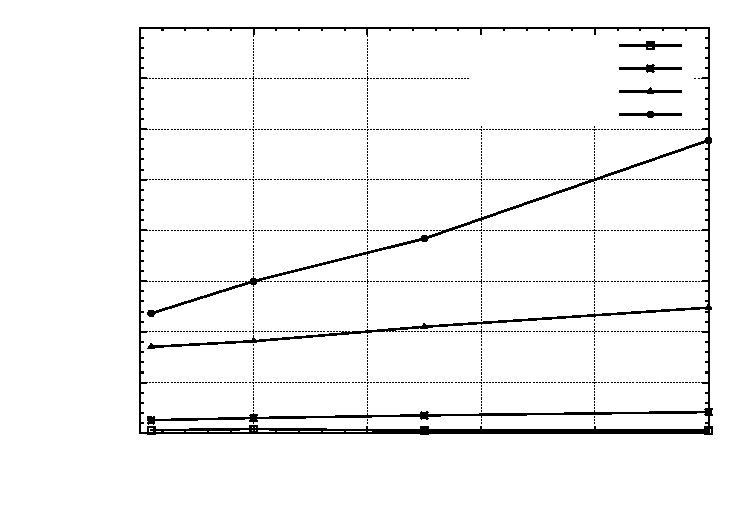
\includegraphics{figures/drift/drift}}%
    \gplfronttext
  \end{picture}%
\endgroup
}
\end{center}

\begin{itemize}
    \item Drift is well controlled at threshold values below 0.01 \AA
    \item Suggests values of 0.001 or 0.005 \AA\ to be the best compromise between speed and accuracy.
\end{itemize}

\end{frame}

% ==========================================================================================
% ==========================================================================================
% ==========================================================================================

\subsection{Statistical impact of the approximation}

% ==========================================================================================
% ==========================================================================================
% ==========================================================================================

\begin{frame}[t]{Statistical impact of the approximation}

\begin{center}
\scalebox{.75}{\input{figures/statddg/statddg}}
\end{center}

\begin{itemize}
    \item Any error introduced by the approximation is below the statistical noise of the MC procedure. 
    \item No statistical dependence was found on the threshold.
\end{itemize}

\end{frame}

% ==========================================================================================
% ==========================================================================================
% ==========================================================================================

\subsection{Chlorine scan}

% ==========================================================================================
% ==========================================================================================
% ==========================================================================================

\begin{frame}[t]{Chlorine scan}

\begin{center}
\scalebox{.75}{% GNUPLOT: LaTeX picture with Postscript
\begingroup
  \makeatletter
  \providecommand\color[2][]{%
    \GenericError{(gnuplot) \space\space\space\@spaces}{%
      Package color not loaded in conjunction with
      terminal option `colourtext'%
    }{See the gnuplot documentation for explanation.%
    }{Either use 'blacktext' in gnuplot or load the package
      color.sty in LaTeX.}%
    \renewcommand\color[2][]{}%
  }%
  \providecommand\includegraphics[2][]{%
    \GenericError{(gnuplot) \space\space\space\@spaces}{%
      Package graphicx or graphics not loaded%
    }{See the gnuplot documentation for explanation.%
    }{The gnuplot epslatex terminal needs graphicx.sty or graphics.sty.}%
    \renewcommand\includegraphics[2][]{}%
  }%
  \providecommand\rotatebox[2]{#2}%
  \@ifundefined{ifGPcolor}{%
    \newif\ifGPcolor
    \GPcolortrue
  }{}%
  \@ifundefined{ifGPblacktext}{%
    \newif\ifGPblacktext
    \GPblacktextfalse
  }{}%
  % define a \g@addto@macro without @ in the name:
  \let\gplgaddtomacro\g@addto@macro
  % define empty templates for all commands taking text:
  \gdef\gplbacktext{}%
  \gdef\gplfronttext{}%
  \makeatother
  \ifGPblacktext
    % no textcolor at all
    \def\colorrgb#1{}%
    \def\colorgray#1{}%
  \else
    % gray or color?
    \ifGPcolor
      \def\colorrgb#1{\color[rgb]{#1}}%
      \def\colorgray#1{\color[gray]{#1}}%
      \expandafter\def\csname LTw\endcsname{\color{white}}%
      \expandafter\def\csname LTb\endcsname{\color{black}}%
      \expandafter\def\csname LTa\endcsname{\color{black}}%
      \expandafter\def\csname LT0\endcsname{\color[rgb]{1,0,0}}%
      \expandafter\def\csname LT1\endcsname{\color[rgb]{0,1,0}}%
      \expandafter\def\csname LT2\endcsname{\color[rgb]{0,0,1}}%
      \expandafter\def\csname LT3\endcsname{\color[rgb]{1,0,1}}%
      \expandafter\def\csname LT4\endcsname{\color[rgb]{0,1,1}}%
      \expandafter\def\csname LT5\endcsname{\color[rgb]{1,1,0}}%
      \expandafter\def\csname LT6\endcsname{\color[rgb]{0,0,0}}%
      \expandafter\def\csname LT7\endcsname{\color[rgb]{1,0.3,0}}%
      \expandafter\def\csname LT8\endcsname{\color[rgb]{0.5,0.5,0.5}}%
    \else
      % gray
      \def\colorrgb#1{\color{black}}%
      \def\colorgray#1{\color[gray]{#1}}%
      \expandafter\def\csname LTw\endcsname{\color{white}}%
      \expandafter\def\csname LTb\endcsname{\color{black}}%
      \expandafter\def\csname LTa\endcsname{\color{black}}%
      \expandafter\def\csname LT0\endcsname{\color{black}}%
      \expandafter\def\csname LT1\endcsname{\color{black}}%
      \expandafter\def\csname LT2\endcsname{\color{black}}%
      \expandafter\def\csname LT3\endcsname{\color{black}}%
      \expandafter\def\csname LT4\endcsname{\color{black}}%
      \expandafter\def\csname LT5\endcsname{\color{black}}%
      \expandafter\def\csname LT6\endcsname{\color{black}}%
      \expandafter\def\csname LT7\endcsname{\color{black}}%
      \expandafter\def\csname LT8\endcsname{\color{black}}%
    \fi
  \fi
  \setlength{\unitlength}{0.0500bp}%
  \begin{picture}(7200.00,5040.00)%
    \gplgaddtomacro\gplbacktext{%
      \csname LTb\endcsname%
      \put(682,440){\makebox(0,0)[r]{\strut{}-6}}%
      \put(682,1059){\makebox(0,0)[r]{\strut{}-4}}%
      \put(682,1679){\makebox(0,0)[r]{\strut{}-2}}%
      \put(682,2298){\makebox(0,0)[r]{\strut{} 0}}%
      \put(682,2917){\makebox(0,0)[r]{\strut{} 2}}%
      \put(682,3536){\makebox(0,0)[r]{\strut{} 4}}%
      \put(682,4156){\makebox(0,0)[r]{\strut{} 6}}%
      \put(682,4775){\makebox(0,0)[r]{\strut{} 8}}%
      \put(1358,220){\makebox(0,0){\strut{}C2}}%
      \put(1903,220){\makebox(0,0){\strut{}C2$^\prime$}}%
      \put(2447,220){\makebox(0,0){\strut{}C3}}%
      \put(2992,220){\makebox(0,0){\strut{}C3$^\prime$}}%
      \put(3536,220){\makebox(0,0){\strut{}C4}}%
      \put(4081,220){\makebox(0,0){\strut{}C4$^\prime$}}%
      \put(4625,220){\makebox(0,0){\strut{}C5}}%
      \put(5170,220){\makebox(0,0){\strut{}C5$^\prime$}}%
      \put(5714,220){\makebox(0,0){\strut{}C6}}%
      \put(6259,220){\makebox(0,0){\strut{}C6$^\prime$}}%
      \put(176,2607){\rotatebox{-270}{\makebox(0,0){\strut{}$\Delta\Delta G_{\textrm{bind}}(\textbf{A} \longrightarrow \textbf{B}$ (kcal/mol)}}}%
    }%
    \gplgaddtomacro\gplfronttext{%
      \csname LTb\endcsname%
      \put(5816,4602){\makebox(0,0)[r]{\strut{}GB/SA (no threshold)}}%
      \csname LTb\endcsname%
      \put(5816,4382){\makebox(0,0)[r]{\strut{}GB/SA (threshold)}}%
      \csname LTb\endcsname%
      \put(5816,4162){\makebox(0,0)[r]{\strut{}TIP4P}}%
    }%
    \gplbacktext
    \put(0,0){\includegraphics{figures/scan/scan}}%
    \gplfronttext
  \end{picture}%
\endgroup
}
\end{center}

\begin{itemize}
    \item Qualitative agreement between GB/SA and TIP4P
    \item GB/SA predicted the same substitution pattern as TIP4P, which produced a highly active compound. (Leung et al, 2010).
\end{itemize}
\end{frame}

% ==========================================================================================
% ==========================================================================================
% ==========================================================================================

\section{Summary}

% ==========================================================================================
% ==========================================================================================
% ==========================================================================================

\begin{frame}{Summary}

\begin{itemize}
    \item It was of interest to be able to employ GB/SA solvation in our efforts towards computer-aided drug design using FEP while maintaining computational efficiency.
    \item FEP was successfully implemented within the GB/SA protocol: test perturbations revealed smooth trajectories of energies and energy components; free energies of solvation with TIP4P were well reproduced with GB/SA, but long simulations of large systems were too slow for practical use.
    \item An approximated generalized Born potential was implemented wherein atom pair energies are only updated after a Monte Carlo move if their Born radii have changed by more than a specified threshold since the last accepted move. By skipping a large number of energy pair calculations, significant speedup was achieved with minimal loss of accuracy.
    \item A chlorine scan used in our search for NNRTIs was performed using our FEP/GBSA protocol and yield results qualitatively similar to those with TIP4P, correctly predicting an active substitution pattern.
\end{itemize}

\end{frame}

\begin{center}
\hspace*{-.35cm}\includegraphics[scale=0.355]{figures/ack.pdf}
\end{center}











\end{document}

% ==========================================================================================
% ==========================================================================================
% ==========================================================================================

\begin{frame}[t]{Frame with columns}

    \begin{columns}

        \begin{column}{0.5\textwidth}

              {\centering col1 \\}
        
        \end{column}
        
        \begin{column}{0.5\textwidth}  
        
              {\centering col2 \\}
        
        \end{column}

    \end{columns}

\end{frame}